\documentclass[11pt, a4paper]{article}
\usepackage{tikz}
\usetikzlibrary{positioning}
\usepackage{natbib}
\usepackage{hyperref}
\usepackage{amsmath,amssymb}
%----------Title Page---------
\title{
    Training Convolutional Neural Networks with Gradient Descent\\~\\
    \large The Impact of LeNet-5 Twenty Five Years After Publication}
\author{
    Maxwell Banks
}
\date{May 9, 2024}
%-----------------------------
\newcommand\fvec[1]{\vec{\textbf{#1}}}
\newcommand\bdot{\boldsymbol{\cdot}}


\begin{document}
\nocite{*}
\maketitle
\newpage

\section{Historical Event}
This historical event analyzed by this paper is the publication of \textit{Gradient-Based Learning Applied to 
Document Recognition} \cite{lecun}. This paper revolutionized the training of neural networks and is the antecedent 
to much of the modern field of machine learning. For a brief primer of the anatomy of a neural network, refer to 
\hyperref[sec:neuralnet]{Appendix A}.

\section{Summary}
The breakout research paper \textit{Gradient-Based Learning Applied to Document Recognition} \cite{lecun}
outlined LeNet-5, one of the first published instances of a Convolutional Neural Network (CNN). CNNs are a subtype
of neural network that generally specialize in image recognition (this is not univerally true, but for brevity this
paper will assume inputs are pixels of an image). \cite{lecun} discusses using gradient-based learning 
techniques to train neural networks in recognizing letters, highlighting a variety of network architectures 
and explaining the effectiveness of gradient-based learning in the context of those architectures. \\

\cite{lecun} had wide-ranging impacts on the field of machine learning as a whole, but perhaps the most 
notable impact was the popularization of CNNs trained using gradient-based learning. As the paper itself notes, 
"Gradient-Based Learning procedures have been used since the late 1950's, but they were mostly limited to 
linear systems." \cite{lecun} The key innovation of \textit{Gradient-Based Learning Applied to Document Recognition} was to apply gradient-based 
learning (specifically, gradient descent) as a training mechanism for CNNs by using gradient descent to determine
the adjustment of node weights by minimizing the "loss function", a function representing how incorrect a neural 
network's guess was.\\

Gradient descent is a technique that dates back to Augustin-Louis Cauchy who outlined the technique in his pamphlet 
\textit{M\'ethode g\'en\'erale pour la r\'esolution des syst\`emes d'\'equations simultan\'ees} \cite{cauchy}. Cauchy described this technique as "...a general 
method which may be able to serve to resolve directly a system of simultaneous equations", and was mostly concerned
with using it to determine the movement of a star with precision. This technique leverages calculus to minimize a system of equations by repeatedly
calculating the gradient (interestingly, the paper itself does not appear to use the term gradient--it exclusively
uses partial derivatives) at a point, then "stepping" in the opposite direction of the gradient to a "lower" point. This 
process is repeated until a minimum is reached. 

\section{Explanation of Enhancement}
\cite{lecun} was a formative paper in the field of machine learning, especially computer vision. Modern CNNs can trace 
their lineage directly back to LeNet-5, and other machine learning architectures are similarly dependent on gradient descent 
as a training model. Because of the performance improvements in training neural nets afforded by \cite{lecun}, image 
recognition is now cheap and fairly ubiquitous--everything from phones to kiosks is capable of analyzing images. \\

There are a multitude of positive advancements that stem from the progeny of LeNet-5, but perhaps the most promising field 
for image recognition is healthcare. Computer vision algorithms are being leveraged to help analyze medical scans and assist 
doctors in finding complications faster and earlier--what takes a doctor hours to scan can be done at a high rate of accuracy
by a neural network in mere seconds. \cite{rana}, a metastudy of forty primary studies, notes that "various 
classical [Machine Learning] and [Deep Learning] techniques are extensively applied [in the healthcare domain] to deal with 
data uncertainty...". This on its own is impressive, but it further goes on to note that "...a series of experiments using 
MRI dataset has provided a comparative analysis of [Machine Learning] classifiers and [Deep Learning] models where CNN (97.6\%) 
and RF (96.93\%) have outperformed other algorithms." \cite{rana} Twenty years after the initial paper, CNNs (and the associated 
gradient descent training mechanism) are more relevant than ever. \\

CheXED is an excellent example of timesaving capabilites of CNNs in the medical field. Developed by researchers at Stanford, 
CheXED scans radiograph images to detect pneumonia and "...required less than a second to identify the findings on a single chest 
radiograph." \cite{irvin} CheXED is not yet capable of independently diagnosing a patient, but it does provide powerful initial 
scan that can then direct doctors to potential problem areas faster. \cite{irvin} concludes that "Integration of CheXED with clinical 
decision support systems like ePNa may help reduce time to diagnosis and improve pneumonia management in the emergency department." \\

Machine learning in healthcare is still in early stages, but stands to save lives by minimizing the turnaround time between inspection 
and diagnosis. At the forefront of this wave of innovation are CNNs, which would not have been possible without the training improvements 
pioneered by \cite{lecun}.


\section{Calculus Steps}
Gradient descent relies on an important principle: \textit{the direction of a gradient evaluated at a 
point is the direction of steepest ascent at that point}. This can be proven trivially from the definition
of a directional derivative, as seen below:
\begin{center}
    \begin{tabular}{l | c | l}
        0 & Find $max(D_{\vec{u}}f)$ at point $P_0$ & Problem\\
        1 & Let $\vec{u}$ be some arbitrary vector & Assumption\\
        2 & Let $\theta$ be the angle between $\vec{u}$ and $\nabla f$ & Assumption \\
        2 & $\fvec{u} = \frac{\vec{u}}{|\vec{u}|}$ & Definition of unit vector\\
        3 & $D_{\vec{u}}f = \nabla f \cdot \fvec{u}$ & Definition of directional der.\\
        4 & $D_{\vec{u}}f = \frac{\nabla f \cdot \vec{u}}{|\vec{u}|}$ & Substitution of line 2 into 3 \\
        5 & $D_{\vec{u}}f = \frac{|\nabla f| |\vec{u}| cos(\theta)}{|\vec{u}|}$ & Definition of dot product \\
        6 & $D_{\vec{u}}f = |\nabla f| cos(\theta)$ & Reduction \\
        7 & $max(cos(\theta)) \rightarrow \{\theta | \theta = 2\pi n, n \in \mathbb{Z}\}$ & Definition of cosine \\
        8 & $max(cos(\theta)) = cos(2\pi n)$ & Extension of line 7 \\
        9 & Let $n = 0$ & Selection based on line 7 \\
        10 & $max(cos(\theta)) = cos(2 \pi n) = cos(0)$ & Substitution of line 9 \\
        11 & $max(D_{\vec{u}}f) = max(|\nabla f| cos(\theta))$ & Identity \\
        12 & $max(D_{\vec{u}}f(P_0)) = max(|\nabla f(P_0)| cos(\theta))$ & Evaluating at point \\
        13 & $max(D_{\vec{u}}f(P_0)) = |\nabla f(P_0)| max(cos(\theta))$ & Pulling out constant \\
        14 & $max(D_{\vec{u}}f(P_0)) = |\nabla f(P_0)| cos(0)$ & Substitution of line 10\\
        15 & $max(D_{\vec{u}}f(P_0)) = |\nabla f(P_0)|$ & Reduction \\
        16 & $max(D_{\vec{u}}f(P_0)) = |\nabla f(P_0)|$ & Result
    \end{tabular}
\end{center}
As demonstrated above, the maximium value of the directional derivative taken at a point is the gradient evaluated at that point.\\

Gradient descent leverages this to know which direction to \textit{avoid}--to go downhill, simply don't go uphill. With that in mind,
we can define the process for gradient descent:

\begin{center}
    \begin{tabular}{l | c | l}
        0 & Move \textit{away} from the direction of steepest ascent & Problem\\
        1 & Let $P$ be an arbitrary starting position & Assumption\\
        2 & Let $\gamma$ be the scalar distance of a step & Assumption\\
        3 & $P_{n+1} = P_n - \gamma \nabla f(P_n)$ & Gradient Descent \\
    \end{tabular}
\end{center}

With the formula for gradient descent defined, we can demonstrate an example:
\begin{center}
    \begin{tabular}{l | c | l}
        0 & Minimize $f$ using gradient descent & Problem\\
        1 & Let $f(x,y)=x^2+y^2$ & Assumption\\
        2 & Let $\gamma = \frac{1}{2}$ & Assumption\\
        3 & Let $P_0 = (2,2)$ & Assumption\\
        4 & $P_{n+1} = P_n - \gamma \nabla f(P_n)$ & Gradient Descent \\
        5 & $P_{1} = (2,2) - \frac{1}{2} \nabla f(P_0)$ & Substituting lines 1,2,3 \\
        6 & $\nabla f = \frac{\partial}{\partial x}f(x,y)\boldsymbol{\hat{\textbf{\i}}} + \frac{\partial}{\partial y}f(x,y)\boldsymbol{\hat{\textbf{\j}}}$ & Definition of gradient \\
        7 & $\frac{\partial}{\partial x}f(x,y) = 2x$ & Reduction \\
        8 & $\frac{\partial}{\partial y}f(x,y) = 2y$ & Reduction \\
        9 & $\nabla f = 2x\boldsymbol{\hat{\textbf{\i}}} + 2y \boldsymbol{\hat{\textbf{\j}}}$ & Substituting lines 7,8 \\
        10 & $\nabla f(P_0) = 2(2)\boldsymbol{\hat{\textbf{\i}}} + 2(2) \boldsymbol{\hat{\textbf{\j}}}$ & Substituting line 3 \\
        11 & $P_{1} = (2,2) - \frac{1}{2} (4\boldsymbol{\hat{\textbf{\i}}} + 4 \boldsymbol{\hat{\textbf{\j}}})$ & Combining lines 5,10 \\
        12 & $P_{1} = (2,2) - (2\boldsymbol{\hat{\textbf{\i}}} + 2 \boldsymbol{\hat{\textbf{\j}}})$ & Reducing \\
        13 & $P_{1} = (0,0)$ & Reducing \\
        14 & $P_{2} = P_1 - \frac{1}{2} \nabla(P_1)$ & Setting up next step \\
        15 & $\nabla f(P_1) = 2(0)\boldsymbol{\hat{\textbf{\i}}} + 2(0) \boldsymbol{\hat{\textbf{\j}}}$ & Substituting from line 9 \\
        16 & $\nabla f(P_1) = 0$ & Reducing \\
        17 & $P_{2} = P_1 - \frac{1}{2} (0)$ & Combining lines 14,16\\
        18 & $P_{2} = P_1$ & Reducing\\
        19 & $P_{2} = P_1$ & Done, converged\\
    \end{tabular}
\end{center}
The process ends when we converge on an answer (this is not always the case, depending on step size we can diverge). In this case the descent
was fairly trivial and took only two iterations, but a more complex function like $f(x,y)=\frac{x^2cos(x)}{16} + \frac{y^2sin(y)}{24}$ would 
likely take more steps (and more room than this paper has...).
\section{What If...}

If the gradient descent calculations had not been done correctly in \cite{lecun}, it is unlikely that the paper would have found any training
improvements of note. In a best-case scenario, the errors would be caught during peer review and the only impact would be a several-month delay 
in the publishing of the paper, with the presumed knock-on effect of delaying our current progress in machine learning by several months.\\

In a worst-case scenario, the paper fails to find anything meaningful and is overlooked. Until some other researcher stumbled upon the idea of 
using gradient descent to teach neural networks (with the \textit{proper} math in place), neural network research would likely have remained 
much less accessible due to the ineffectiveness of training techniques. As a result, many common staples of today's technology such as image 
recognition would be underdeveloped, with unpredictable but certainly negative economic impacts. \\

The most concerning second-order effects would be to the medical advancements mentioned above--current cutting-edge medical machine learning 
applications rely heavily on gradient descent. Any delay to the development of these technologies indirectly harms future patients by reducing 
their potential quality of care. As such, in a worst-case scenario incorrect calculations in \cite{lecun} would cost lives, and conversely the 
correct calculations may well turn out to save lives.

\newpage
\bibliographystyle{apalike}
\bibliography{bibliography}

\newpage
\appendix
\section{Appendix: How a Neural Network Works}
\label{sec:neuralnet}
Neural networks are a machine learning architecture commonly used for pattern recognition. Named for their 
similarity to human brains, traditional neural networks are composed of groups of nodes (called 
\textit{layers} of \textit{neurons}). Each node in a layer is connected to nodes in the preceding and following
layers, and contains some innate value (called a \textit{weight}). To process data with a neural network, data
is broken into discrete chunks that are fed into the first (input) layer of neurons. These neurons mutate the 
input according to their weight, then pass the result to the next (hidden) layer to continue the process. This 
process continues until the final (output) layer, wherein each node outputs a single number. These numbers can 
be used to classify inputs--for example, a neural net classifying images into "dog" or "cat" might have two
output nodes $O_1$ and $O_2$ corresponding to "dog" and "cat" respectively. The classification of an image into
"dog" or "cat" would be decided by $max(O_1, O_2)$. \\
\begin{center}
    \textbf{A Simple Diagram of a Neural Network}\\
    

\tikzset{%
  every neuron/.style={
    circle,
    draw,
    minimum size=1cm
  },
  neuron missing/.style={
    draw=none, 
    scale=4,
    text height=0.333cm,
    execute at begin node=\color{black}$\vdots$
  },
}

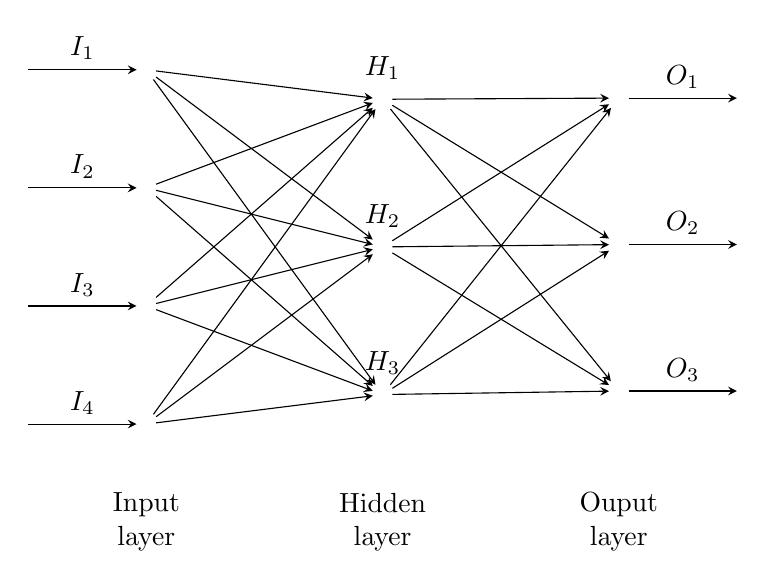
\begin{tikzpicture}[x=1.5cm, y=1.5cm, >=stealth]

\foreach \m/\l [count=\y] in {1,2,3,4}
  \node [every neuron/.try, neuron \m/.try] (input-\m) at (0,2.5-\y) {};

\foreach \m [count=\y] in {1,2,3}
  \node [every neuron/.try, neuron \m/.try ] (hidden-\m) at (2,2.5-\y*1.25) {};

\foreach \m [count=\y] in {1,2,3}
  \node [every neuron/.try, neuron \m/.try ] (output-\m) at (4,2.5-\y*1.24) {};

\foreach \l [count=\i] in {1,2,3,4}
  \draw [<-] (input-\i) -- ++(-1,0)
    node [above, midway] {$I_\l$};

\foreach \l [count=\i] in {1,2,3}
  \node [above] at (hidden-\i.north) {$H_\l$};

\foreach \l [count=\i] in {1,2,3}
  \draw [->] (output-\i) -- ++(1,0)
    node [above, midway] {$O_\l$};

\foreach \i in {1,...,4}
  \foreach \j in {1,...,3}
    \draw [->] (input-\i) -- (hidden-\j);

\foreach \i in {1,...,3}
  \foreach \j in {1,...,3}
    \draw [->] (hidden-\i) -- (output-\j);

\foreach \l [count=\x from 0] in {Input, Hidden, Ouput}
  \node [align=center, below] at (\x*2,-2) {\l \\ layer};

\end{tikzpicture}


\end{center}

\end{document}